\documentclass{article}
\usepackage[left=2cm,right=2cm,top=3cm,bottom=3cm,letterpaper]{geometry}
\usepackage[spanish]{babel}
\usepackage[utf8]{inputenc}
\usepackage{amsmath}
\usepackage{graphicx}

\title{Almacenes y Minería de Datos \\Proyecto Final\\ Entregable 1}
\author{Adolfo Marín Arriaga\\Juan Carlos López López\\Luis Rodrigo Rojo Morales}
\date{\today\\}

\begin{document}
 \maketitle
 
 {\bf Algoritmo 1: Naive Bayes}\\
 
 {\bf Objetivo}\\
 
 El objetivo de Naive Bayes o Clasificador bayesiano ingenuo es la construccion de clasificadores en base a datos que ya se conocen por ejemplo clasificar si una persona es hombre o mujer basandose
 en los datos que se tienen de su altura, peso y tamaño del pie. Se usa basandose en el teorema de Bayes y asume que las variables que se usan para predecir son 
 independientes\\
 
 {\bf Descripción}\\
 
 Lo que tenemos es un objeto que es lo que se quiere clasificar, las variables que se van a usar para predecir que son los datos que ya conocemos y distintas clases a donde podria 
 ir cada objeto después de la clasificación. Se usa la regla de bayes que dice que si se tienen 2 eventos A y B se saca la probabilidad de A dado B como:
 $$ P(A \mid B) = \frac{P(B \mid A) \, P(A)}{P(B)} $$
 \begin{itemize}
  \item $P(A \mid B)$ Es la probabilidad de que se cumpla  A dado B, es la probabilidad a posteriori.
  \item $P(B \mid A)$ Es la probabilidad de B dado que se cumple A.
  \item $P(A)$ y $P(B)$ Son las probabilidades que se cumplan A y B respectivamente, estas son la probabilidad a priori
 \end{itemize}
 Para el clasificador bayesiano ingenuo hay distintas clases en las que puede caer un objeto después de ser clasificado y distintas variables predictivas, entonces
 si tenemos un conjunto de variables predictivas $X=\{x_1,...,x_n\}$ y m clases para la clasificación $C_1,...,C_m$, el clasificador dice que la 
 probabilidad de que un objeto pertenezca a la clase $C_k$ se calcula como:
 \begin{equation*}
 p(C_k|X)=\frac{1}{Z}p(C_k)\prod_{i=1}^{n}p(x_i|C_k)
 \end{equation*}
 \begin{itemize}
  \item $X$ es el conjunto de variables predictivas $X=\{x_1,...,x_n\}$.
  \item $C_k$ es una clase de $C_1,...,C_m$
  \item $Z$ es igual a un factor que depende solo de $x_1,...,x_n$, es una constante si sus valores son conocidos
 
 \end{itemize}
{\bf Ejemplo:}\\
 
 Un ejemplo es si queremos clasificar frutas, las clases son platano, naranja y otras, se hizó un conjunto de entrenamiento con las variables
 de longitud, sabor y color y nos dio que:
 \begin{center}
  \begin{tabular}{|l||l|l||l|l||l|l||l|}
   \hline
   Fruta & Alargada & No Alargada & Dulce & No Dulce & Amarilla & No Amarilla & Total \\ \hline \hline
   Platano & 400 & 100 & 350 & 150 & 450 & 50 & 500 \\ \hline
   Naranja & 0 & 300 & 150 & 150 & 300 & 0 & 300 \\ \hline
   Otras & 100 & 100 & 150 & 50 & 50 & 150 & 200 \\ \hline \hline
   Total & 500 & 500 & 650 & 350 & 800 & 200 & 1000 \\ \hline
  \end{tabular}
  \end{center}
  Ahora queremos predecir en que clase cae una nueva fruta que llega y es amarilla, alargada y dulce.
  Calculamos las probabilidades:
  \begin{itemize}
   \item $ P(platano) = 500/1000 = $0.5
   \item $ P(platano \mid alargada) = \frac{P(alargada \mid platano) \, P(platano)}{P(alargada)} = \frac{400/500 \, \cdot 500/1000}{500/1000} = $0.8
   \item $ P(platano \mid dulce) = \frac{P(dulce \mid platano) \, P(platano)}{P(dulce)} = \frac{350/500 \, \cdot 500/1000}{650/1000} = $0.5384
   \item $ P(platano \mid amarilla) = \frac{P(amarilla \mid platano) \, P(platano)}{P(amarilla)} = \frac{450/500 \, \cdot 500/1000}{800/1000} = $0.5625
   \item $ P(naranja) = 300/1000 = $0.3
   \item $ P(naranja \mid alargada) = \frac{P(alargada \mid naranja) \, P(naranja)}{P(alargada)} = \frac{0/300 \, \cdot 300/1000}{500/1000} = $0
   \item $ P(naranja \mid dulce) = \frac{P(dulce \mid naranja) \, P(naranja)}{P(dulce)} = \frac{150/300 \, \cdot 300/1000}{650/1000} = $0.2307
   \item $ P(naranja \mid amarilla) = \frac{P(amarilla \mid naranja) \, P(naranja)}{P(amarilla)} = \frac{300/300 \, \cdot 300/1000}{800/1000} = $0.375
   \item $ P(otras) = 200/1000 = $0.2
   \item $ P(otras \mid alargada) = \frac{P(alargada \mid otras) \, P(otras)}{P(alargada)} = \frac{100/200 \, \cdot 200/1000}{500/1000} = $0.2
   \item $ P(otras \mid dulce) = \frac{P(dulce \mid otras) \, P(otras)}{P(dulce)} = \frac{150/200 \, \cdot 200/1000}{650/1000} = $0.2307
   \item $ P(otras \mid amarilla) = \frac{P(amarilla \mid otras) \, P(otras)}{P(amarilla)} = \frac{50/200 \, \cdot 200/1000}{800/1000} = $0.0625
  \end{itemize}
  Ahora para el clasificador con su fórmula:
  \begin{itemize}
   \item $p(platano|alargada,dulce,amarilla)=\frac{1}{Z}p(platano)p(platano|alargada)p(platano|dulce)p(platano|amarilla)$ \\=
   $\frac{1}{Z}$0.5 $\cdot$ 0.8 $\cdot$ 0.5384 $\cdot$ 0.5625 = $\frac{1}{Z}$0.121147
   \item $p(naranja|alargada,dulce,amarilla)=\frac{1}{Z}p(naranja)p(naranja|alargada)p(naranja|dulce)p(naranja|amarilla)$ \\=
   $\frac{1}{Z}$0.5 $\cdot$ 0 $\cdot$ 0.2307 $\cdot$ 0.375 = $\frac{1}{Z}$0
   \item $p(otras|alargada,dulce,amarilla)=\frac{1}{Z}p(otras)p(otras|alargada)p(otras|dulce)p(otras|amarilla)$ \\=
   $\frac{1}{Z}$0.2 $\cdot$ 0.2 $\cdot$ 0.2307 $\cdot$ 0.0625 = $\frac{1}{Z}$0.00057675
  \end{itemize}
  Conocemos la probabilidad de que lo que recibamos sea dulce, alargado y amarillo entonces tomamos $Z$ como:
  \begin{itemize}
   \item $p(alargada)p(dulce)p(amarilla) = \frac{500}{1000}\cdot\frac{650}{1000}\cdot\frac{800}{1000}$=0.26
  \end{itemize}
  Entonces reemplazando $Z$
  \begin{itemize}
   \item $p(platano|alargada,dulce,amarilla) = \frac{0\ldotp121147}{0\ldotp26}$=0.46595
   \item $p(naranja|alargada,dulce,amarilla) = \frac{0}{0\ldotp26}$=0
   \item $p(otras|alargada,dulce,amarilla) = \frac{0\ldotp00057675}{0\ldotp26}$=0.2218
  \end{itemize}
  La probabilidad mas grande es la de que sea platano, entonces si llega una fruta que sea alargada, dulce y amarilla la clasificamos como que va a ser un 
  platano.\\
  
{\bf Bibliografía}
\begin{itemize}
 \item https://en.wikipedia.org/wiki/Naive\_Bayes\_classifier
 \item https://en.wikipedia.org/wiki/Bayes\%27\_theorem
\end{itemize}

{\bf Plan de trabajo}\\

Para nuestro problema en el preprocesamiento de datos es necesario hacer limpieza en los campos workclass, occupation y native-country, porque en algunas
filas tienen un ? en vez de alguno de los datos de las opciones que se dan. \\
\begin{center}
 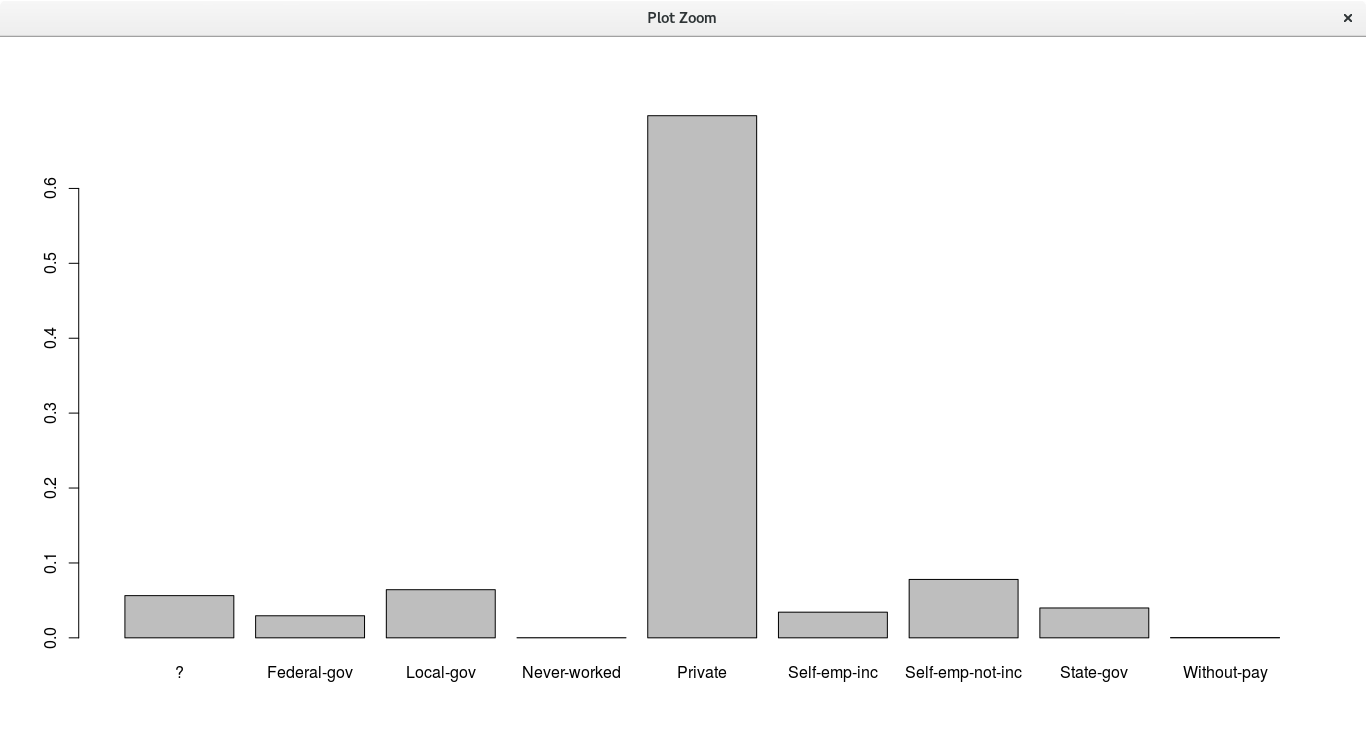
\includegraphics[scale=0.3]{trabajos}\\
\end{center}

También para los datos que son numéricos los datos varian en muchos valores por ejemplo
edades tiene 71 valores distintos, entonces para estos valores numéricos para que no halla tantas probabilidades, lo mejor para hacer naive bayes seria hacer 
discretización de los valores numéricos como por ejemplo con binning para tomarlos por rangos. Así en vez de tomar los 71 valores posibles de edades, tomaría una
menor cantidad de rangos.\\
\begin{center}
 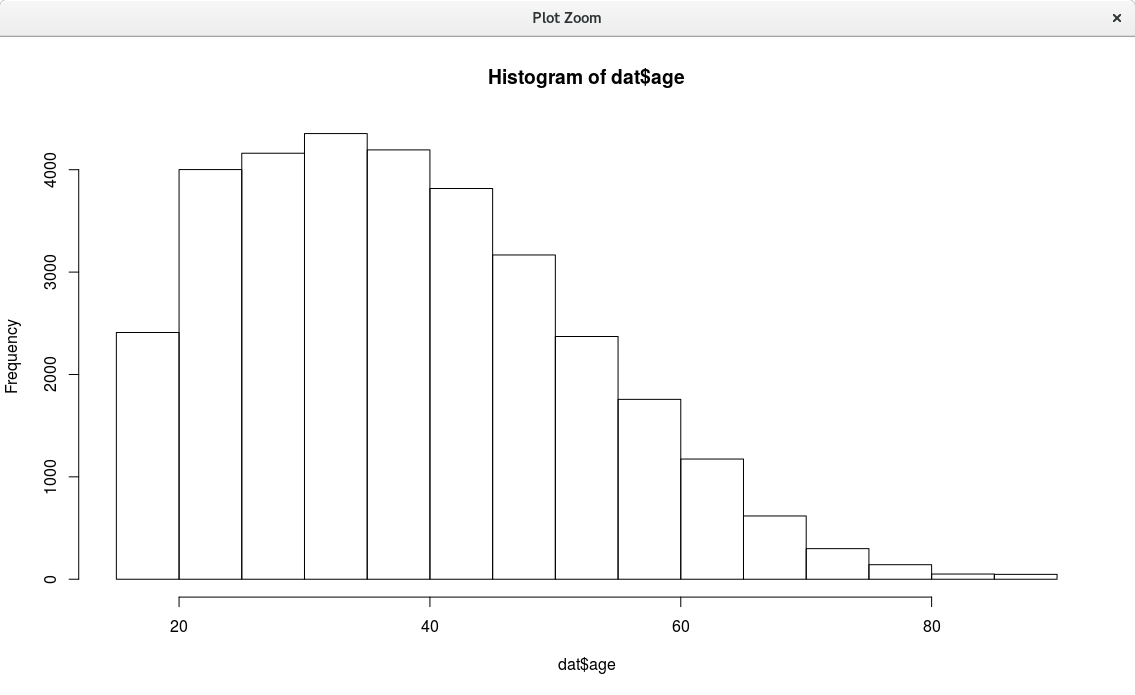
\includegraphics[scale=0.3]{edades}\\
\end{center}
Los datos que no son númericos si caen en opciones predefinidas por lo que salvo los campos que tienen valores con ? no hay inconsistencias en estos datos.
También otros problemas que hay en los datos que son numéricos es que hay muchos outliers, por ejemplo en horas a la semana la mayoria trabaja alrededor de 40
pero hay datos que van desde 1 hasta 99.\\
\begin{center}
 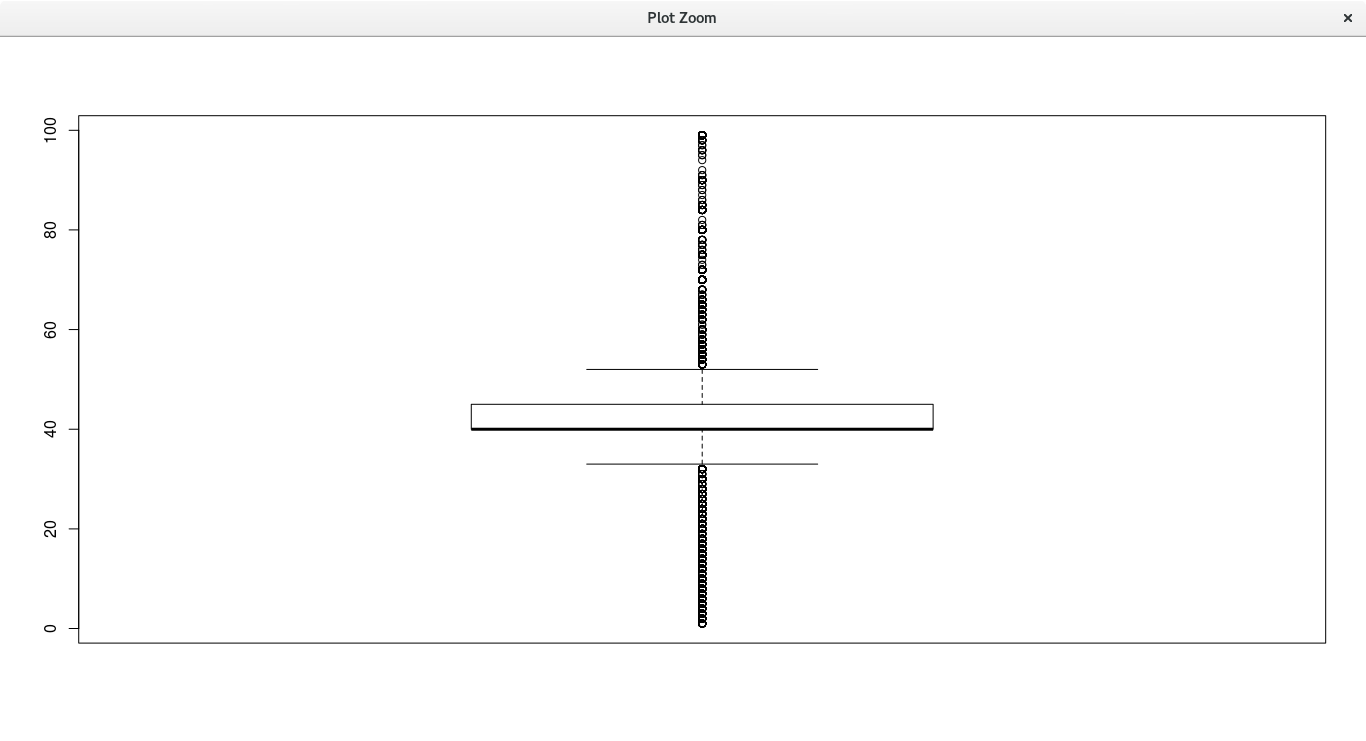
\includegraphics[scale=0.3]{horas}\\
\end{center}
En este caso los outliers se podrían en rangos que sean mayor que un valor y menor que un valor en la discretización que se había planteado previamente.
 
\end{document}
